\documentclass[11pt]{article}

%!TEX root = ../project_description/project_description.tex
\usepackage[USenglish]{babel}

\usepackage[T1]{fontenc}      
\usepackage[utf8]{inputenc}

\usepackage{amsmath,amsthm}
\usepackage{amsfonts}
\usepackage{amssymb}
\usepackage{stmaryrd}
\usepackage{graphicx}
% \usepackage{titlesec}
\usepackage[margin=1in]{geometry}
\usepackage{subcaption}

\usepackage{xspace}
\newcommand{\ie}{i.e.\@\xspace}
\newcommand{\eg}{e.g.\@\xspace}

\makeatletter
\newcommand*{\etc}{%
    \@ifnextchar{.}%
        {etc}%
        {etc.\@\xspace}%
}
\makeatother

\makeatletter
\newcommand*{\etal}{%
    \@ifnextchar{.}%
        {et al}%
        {et al.\@\xspace}%
}
\makeatother

% \titleformat{\subsubsection}[runin]{\normalfont\large\bfseries}{\thesubsubsection}{1em}{}[]

\usepackage[textsize=scriptsize]{todonotes}

% \newlength{\arrow}
% \settowidth{\arrow}{\scriptsize$1000$}
\newcommand*{\goesto}[1]{\xrightarrow{#1}}
\newcommand*{\Xbar}{\overline{X}}
\newcommand*{\xbar}{\overline{x}}

\usepackage{hyperref}
\usepackage{listliketab}
\usepackage{array}
\usepackage{longtable}
\usepackage{enumitem}
\usepackage{sectsty}
\usepackage{url}
\usepackage{bibentry}
\usepackage{fancyhdr}
\usepackage{xparse}

\newenvironment{thoughts}{\begin{itemize}[itemsep=0pt]}{\end{itemize}}
\newcommand{\athought}[1]{\item \emph{#1}}

\RequirePackage[final]{microtype}
\DisableLigatures{encoding = T1, family = tt* }

\bibliographystyle{plain}


% \usepackage{minted}
% \newminted{haskell}{}
% \newmintinline[hask]{haskell}{}

\usepackage{listings}
\usepackage{xcolor}

\definecolor{mygreen}{rgb}{0,0.6,0}
\definecolor{mygray}{rgb}{0.5,0.5,0.5}
\definecolor{mymauve}{rgb}{0.58,0,0.82}

\lstset{ 
  % backgroundcolor=\color{white},   % choose the background color; you must add \usepackage{color} or \usepackage{xcolor}; should come as last argument
  basicstyle=\ttfamily,        % the size of the fonts that are used for the code
  flexiblecolumns=true,
  breakatwhitespace=false,         % sets if automatic breaks should only happen at whitespace
  breaklines=true,                 % sets automatic line breaking
  commentstyle=\color{mygreen},    % comment style
  keepspaces=true,                 % keeps spaces in text, useful for keeping indentation of code (possibly needs columns=flexible)
  keywordstyle=\color{blue},       % keyword style
  language=Haskell,                 % the language of the code
  stringstyle=\color{mymauve},     % string literal style
}

% From: https://tex.stackexchange.com/questions/89574/language-option-supported-in-listings
\lstdefinelanguage{JavaScript}{
  keywords={typeof, new, true, false, catch, function, return, null, catch, switch, var, if, in, while, do, else, case, break},
  keywordstyle=\color{blue}\bfseries,
  ndkeywords={class, export, boolean, throw, implements, import, this},
  ndkeywordstyle=\color{darkgray}\bfseries,
  identifierstyle=\color{black},
  sensitive=false,
  comment=[l]{//},
  morecomment=[s]{/*}{*/},
  commentstyle=\color{purple}\ttfamily,
  stringstyle=\color{red}\ttfamily,
  morestring=[b]',
  morestring=[b]"
}

\newcommand{\bnfalt}{\;\mathrel{\mid}\;}
\newcommand{\bnfdef}{%
  \mathrel{\!\colon\!\!\colon\!\mathord{=}}%
}

\newenvironment{centeredlstlisting}
  {%
    \begin{center}
    \begin{tabular}{c}
    \begin{lstlisting}
  }
  {%
    \end{lstlisting}
    \end{tabular}
    \end{center}
  }

\begin{document}

    \setcounter{page}{1}
    \def\title{Project Description}
    %!TEX root = ../project_description/project_description.tex
\begin{center}
    {\Large {\bf Collaborative Research: FET: Small: RUI:\\[1ex]Functional Reactive Molecular Programming}}
\end{center}

\begin{center}
    {\Large \title}
\end{center}


    % %!TEX root = project_description.tex

%%%%%%%%%%%%%%%%%%%%%%%%
\section{Introduction}
\label{sec:introduction}
%%%%%%%%%%%%%%%%%%%%%%%%
Molecular programming harnesses the reactivity of molecules to perform directed computations at the nanoscale.
Leonard Adleman was the first to demonstrate the feasibility of molecular programming by solving instances of the Hamiltonian path problem with DNA biomolecules and common enzyme reactions~\cite{adleman94}.
Since Adleman's initial work, molecular programming techniques have rapidly progressed.
Today, virtually any two- or three-dimensional nanostructure can be compiled into biomolecules that spontaneously self-assemble the target structure with nanometer precision~\cite{jRoth06,jDDLHGS09,jDMTVCS09,jKOSY12,benson2015dna,Juneaav0655}.
Specific biomolecules such as DNA are also being explored for data archival purposes because of their longevity, information density, and rapidly decreasing synthesis costs~\cite{jChGaKo12,jGBCDLSB13,hughes17}.
Molecular programming techniques are also employed to construct dynamic molecular machines for transporting nanoscale cargo~\cite{jShiPie04,jDoBaCh12,jWoodsQian17} as well as amorphous molecular computations that naturally interface with existing biological systems~\cite{cKiHoWi05,jQiaWin11a,jCDSPCS13}.

The underlying theory of molecular programming is also rapidly advancing and helping to inform the experimental results.
Erik Winfree's tile self-assembly model~\cite{oWinf98,jWeDaYi12,qian17} sparked the interest of many computer scientists in 1998 and is still an actively investigated model today~\cite{jLaLuSu09,cDLPSW10,jMeunier17,cFuSuWe19}.
One of the most prominent models of molecular programming is the chemical reaction network, which is a mathematical abstraction of chemical kinetics used for over a half century~\cite{jAris65}.
Chemical reaction networks are a natural bridge between the theory and practical applications of molecular programming.
In theory, they are algorithmically universal~\cite{jSCWB08,cFLBP17} and can be automatically compiled into concrete DNA molecules that simulate their behavior with arbitrary precision~\cite{cSoSeWi09,jLYCP12,jCard13,jCDSPCS13,jSPSWS17,cBSJDTW17}.
As a result, chemical reaction networks are regarded as a prescriptive programming language for deploying algorithms at the nanoscale~\cite{jSCWB08,cSWBG19,jHKLLL18,rdc} and have the potential to accelerate the development the aforementioned biotechnologies.

Roughly, a chemical reaction network (CRN) is a collection of \emph{reactions} over a finite set of abstract molecule types called \emph{species}.
Depending on the target environment, a CRN is either modeled stochastically or deterministically.
Stochastic CRNs are used for modeling molecular reactions in small-volume environments such as \emph{in vivo} experiments and are equivalent to well-known discrete models of computation such as vector addition systems~\cite{oGins66,jKaMiWi67,jKarMil69,jNash73,jLero10,cLero12} and Petri nets~\cite{oPetr62,jMura89,oDavAll10,oReis13}.
Deterministic CRNs are used to model chemical reactions in large-volume environments and are equivalent to Shannon's general purpose analog computer~\cite{jShan41,jGraCos03,jGrac04,cBoGrPo16,cFLBP17,rtcrn2}.

Molecular computation is significantly different from classical computing models and has various advantages and disadvantages.
For example, stochastic CRNs can be regarded as massively parallel distributed computing systems and are closely related to population protocols~\cite{jAADFP06,jAAER07,jAnAsEi08,jAnAsEi08a,Doty2018}.
Their probabilistic nature is harnessed to simulate arbitrary probability distributions and deploy probabilistic algorithms at the nanoscale~\cite{jCaKwLa18,jCOAW19,cWinfe19}.
In fact, the probabilistic semantics of stochastic CRNs is necessary for Turing-complete computation; only semi-linear functions can be computed with probability 1~\cite{cChDoSo12,cCuDoSo14,Doty2015,doty19}.
Programming with molecular reactions also enables programmers to seamlessly interface complex decision processes with existing biological systems, and various cell-to-cell molecular communication protocols are actively being investigated~\cite{jPieAky10,jFYECG16,jChou19}.
% Although current methods for molecular programming are not expected to surpass silicon processing efficiency, the techniques have the potential to broadly impact biomedicine research~\cite{jorge2018overview}.

The unique nature of molecular computation introduces new challenges for programmers.
Molecular reactions are \emph{always active}, which makes even simple sequential tasks challenging to achieve without significant overhead.
Moreover, combining two molecular programs can lead to unexpected interactions, race conditions, and other unwanted side effects.
For example, consider the CRNs from Figure~\ref{fig:min_max_example} (a) and (b) that compute the \( \min(x_1, x_2) \) and \( \max(x_1, x_2) \) functions, respectively.
\begin{figure*}[t!]
    \centering
    \begin{subfigure}[t]{0.23\textwidth}
        \centering
        \begin{minipage}[t][1.5in][b]{0.23\textwidth}
            \vspace*{\fill}
            \[
                X_1 + X_2 \goesto{} Y
            \]
            \vspace*{\fill}
        \end{minipage}
        \vspace*{-1.5em}
        \caption{}
    \end{subfigure}
    ~
    \begin{subfigure}[t]{0.23\textwidth}
        \centering
        \begin{minipage}[t][1.5in][b]{0.23\textwidth}
            \vspace*{\fill}
            \begin{align*}
                X_1 &\goesto{} A_1 + Y\\
                X_2 &\goesto{} A_2 + Y\\
                A_1 + A_2 &\goesto{} B\\
                Y + B &\goesto{} \emptyset
            \end{align*}
            \vspace*{\fill}
        \end{minipage}
        \vspace*{-1.5em}
        \caption{}
    \end{subfigure}
    ~
    \begin{subfigure}[t]{0.23\textwidth}
        \centering
        \begin{minipage}[t][1.5in][b]{0.23\textwidth}
            \vspace*{\fill}
            \begin{align*}
                X_1 &\goesto{} A_1 + Z\\
                X_2 &\goesto{} A_2 + Z\\
                A_1 + A_2 &\goesto{} B\\
                Z + B &\goesto{} \emptyset\\
                X_3 + Z &\goesto{} Y
            \end{align*}
            \vspace*{\fill}
        \end{minipage}
        \vspace*{-1.5em}
        \caption{}
    \end{subfigure}
    ~
    \begin{subfigure}[t]{0.23\textwidth}
        \centering
        \begin{minipage}[t][1.5in][b]{0.23\textwidth}
            \vspace*{\fill}
            \begin{align*}
                X_1 &\goesto{} A_1 + Z\\
                X_2 &\goesto{} A_2 + Z\\
                A_1 + A_2 &\goesto{} B\\
                Z + B &\goesto{} \emptyset\\
                X_3 + Z &\goesto{} Y + W\\
                Y + W + B &\goesto{} X_3
            \end{align*}
            \vspace*{\fill}
        \end{minipage}
        \vspace*{-1.5em}
        \caption{}
    \end{subfigure}
    \caption{\label{fig:min_max_example}
        (a) Computes \( y = \min(x_1, x_2) \), (b) computes \( y = \max(x_1,x_2) \), (c) attempts to compute \( y = f(x_1, x_2, x_2) \) but fails, (d) correctly computes \( y = f(x_1, x_2, x_3) \).
    }
\end{figure*}
The minimum function proceeds by consuming \( X_1 \) and \( X_2 \) molecules until the smaller of the two reactants is completely consumed; the minimum of the two reactants is then produced directly as a result.
In contrast, the maximum function proceeds by computing the sum of reactants $X_1$ and $X_2$ in product $Y$ and then subtracting the minimum of the two reactants (stored in $B$) from $Y$.

In isolation, each CRN correctly computes its respective function, storing its result in species \( Y \).
However, composing the CRNs together to compute a compound function such as
\begin{equation}\label{eq:min_max_function}
    f(x_1, x_2, x_3) = \min(\max(x_1, x_2), x_3)
\end{equation}
results in a race condition that causes the computation to fail.
Figure~\ref{fig:min_max_example}(c) attempts to compute \( f(x_1, x_2, x_3) \) by composing the CRNs (a) and (b) directly.
However, the reaction \( X_3 + Z \goesto{} Y \) prematurely consumes \( Z \)s before the maximum function stabilizes to its final value, causing failure.

Resolving the race condition requires making the offending reaction reversible so that the unwanted side effects can be undone, as shown in Figure~\ref{fig:min_max_example}(d).
Here, we form the composition of the two functions by combining the functions' respective CRNs but with some modifications.
In addition to computing the minimum of $X_3$ and $Z$ directly as the product $Y$, we also generate a residual product $W$.
This product is used in the final reaction in conjunction with the residual reactant $B$ from the maximum computation to restore any $X$s that were consumed prematurely.

Composing CRNs together is only a safe operation if their outputs are produced in a non-decreasing manner~\cite{jCKRS18,doty19}.
Because the output of \( \max(x_1, x_2) \) is produced using a subtraction operation, its output cannot be safely used in downstream computations without carefully ensuring that any reactions consuming its result are reversible.
This reality stymies our attempts at building higher-level programming abstractions since these abstractions rely heavily on the composability of functionality.
Moreover, CRNs are tightly coupled systems, and avoiding such unintended race conditions and side effects is challenging.
Even in systems with only 20 reactions and four species, most species have a chain of dependencies that can be broken by the addition of a single reaction that affects one of its dependencies.
For this reason, molecular programs defined using the CRN syntax are challenging to develop and debug.

To solve these issues, researchers have investigated linguistic support for molecular programming.
For example, Visual GEC~\cite{jPedPhi09}, Visual DSD~\cite{jLYPEP11}, CRN++~\cite{Vasic2020}, and Kaemika~\cite{cardelliKaemika} all define languages for specifying molecular programs.
Visual GEC is concerned with synthetic biology, and its language is based on promoters, ribosome binding sites, protein coding regions and terminators.
Visual DSD is explicitly designed for specifying DNA strand displacement networks.
Kaemika is a chemical reaction network simulator that also includes a language for specifying reactions that extends the notation of chemical reactions with functional programming constructs, in effect, a macro-system for quickly building up chemical reactions.
While the languages defined in these tools work well for their domains, they provide low-level programming constructs that make the development difficult.
Even with the help of tools, it is easy to make subtle mistakes in programs that may be intermittent and difficult to find and debug.
In contrast, CRN++ is a high-level language that gives molecular programmers the ability to specify programs in a more familiar imperative style.
The techniques used in this paper serialize computations in order to achieve this effect, which is a severe restriction on what is, otherwise, an inherently parallel system.

In short, the prior work either (a) provides little support for programming rich, complex molecular systems, or (b) chooses abstractions that hide the essence of CRNs, trading ease of use by limiting their behavior.
We instead recognize the inherent difficulties that CRN's unique computational behavior presents and choose instead to adopt abstractions that allow us to reason about this behavior in a direct, structured manner.
To this end, we propose the construction of a foundations-based programming language for molecular programming based on \emph{functional reactive programming}~(\emph{FRP}), noting that a chemical reaction network is inherently \emph{reactive} in nature.
Functional reactive programming is an established programming paradigm within the programming languages community that directly applies to the task of writing molecular programs~\cite{elliott1997, czaplicki2013, finkbeiner2019, jeffrey2012}.
Furthermore, the analysis of functional reactive programming languages is also well-studied, giving us immediate in-roads for analyzing CRNs written with this language.
For example, Linear Temporal Logic (LTL)~\cite{pnueli1997,manna2012temporal,oBaiKat08} is frequently used to verify the correctness of CRNs~\cite{jKwiTha14,cEHKLLL14,jEKLLLM17}.
By the Curry-Howard Isomorphism, we can view LTL as a type system for our FRP-based language for CRNs.
In this system, whenever a CRN successfully typechecks, we know that it validates its corresponding LTL specification (the LTL specification \emph{is} its type).
Other adaptations from the programming languages are also possible, \eg, program synthesis with LTL specifications~\cite{finkbeiner2019}, further demonstrating the power of this foundations-based approach.

\textbf{Intellectual Merit.}
We propose the design and study of: (1) The syntax and semantics of functional reactive programming languages for both deterministic and stochastic chemical reaction networks, (2) an LTL-inspired type system for these FRP languages, and (3) additional tool-based support for programming CRNs in this FRP style, including development environments and program synthesis techniques.
Reimagining molecular systems as functional reactive programs has the potential to help overcome the unique challenges and complexities of molecular programming.
In particular, this FRP offers to help researchers focus on harnessing the natural strengths of molecular programming rather than focus on avoiding its weaknesses.
Embedding type systems that statically guarantee temporal properties also promises to help ensure these molecular programs are correct, safe, and reliable.
Not only will this proposed work help to advance knowledge into the field of molecular programming, it may reveal insights into related fields such as analog computing and distributed algorithms.

This proposal is organized into the following sections.
Section~\ref{sec:frp_background} provides a light introduction into the functional reactive programming paradigm.
Since the semantics and use of deterministic CRNs and stochastic CRNs are fundamentally dissimilar, we separate our proposed work into two main sections.
In particular, Sections~\ref{sec:frp_dcrns} and~\ref{sec:frp_scrns} details our FRP language design plans for deterministic CRNs and stochastic CRNs, respectively.
Section~\ref{sec:software_support} overviews our plans for developing software support for these languages.
Sections~\ref{sec:broader_impacts} and~\ref{sec:timeline} include more information on the broader impacts and the timeline of the proposed work.
Finally, Section~\ref{sec:prior_nsf_support} is an overview of the PIs' prior NSF support.

% Intellectual Merit: The Intellectual Merit criterion encompasses the potential to advance knowledge; and
%   1. What is the potential for the proposed activity to: Advance knowledge and 
%      understanding within its own field or across different fields?
%   2. To what extent do the proposed activities suggest and explore
%      creative, original, or potentially transformative concepts?
%   3. Is the plan for carrying out the proposed activities well-reasoned,
%      well-organized, and based on a sound rationale? Does the plan incorporate
%      a mechanism to assess success?
%   4. How well qualified is the individual, team, or organization to conduct
%      the proposed activities?
%   5. Are there adequate resources available to the PI (either at the home
%      organization or through collaborations) to carry out the proposed activities?

%%%%%%%%%%%%%%%%%%%%%%%%%%%%%%%%%%%%%%%%%%%%%%%%%%%%%%%%%%%%%%%%%%%%%%%%%%%%%%%%%%%%%%5

% Proposed outline of the rest of the paper
%
% 1. Introduction
%     * Mostly stays the same
%     * Proposed work has four main thrusts:
%        A. Develop FRP languages for both deterministic and stochastic
%           CRN models
%        B. Enrich these languages with STL/LTL typing
%        C. Explore a more advanced FRP approach to stochastic CRNs
%           with signals Time -> Dist State and CSL typing
%        D. Develop IDE tooling support that harnessees these language
%           features, streamlines the development process, and performs
%           static type verification
%
% 2. Functional Reactive Programming
%     * Give background information about FRP while tying it into
%       concepts of CRNs throughout
%
% 3. FRP and Deterministic CRNs
%     * Briefly introduce the input/output deterministic CRN model
%     * Draw connections between between the previous works on
%       chemical circuits and finite automata and FRP
%     * In particular, emphasize how these CRNs are literally signal
%       functions in the FRP sense that transform one type of signal
%       into another
%     * Drawing connections with how real biological systems use
%       molecular communication and react to input signals changing
%       such as the cell cycle switch
%     * Overview Ally's work on deterministic CRNs, the IOCRN type,
%       the Arrow implementations, and examples
%     * Show how the NAND gate and S-R latch can easily be implemented
%       in this characterization. Use the Yampa Arrow syntax to
%       demonstrate how the S-R latch can be implemented using
%       two NAND gates and the Arrow combinators
%     * Emphasize how the Bool type encapsulates the idea of a dual
%       rail encoding whereas the Double type is a continuous real
%       valued signal
%     * Discuss how STL (a continuous-space variant of LTL) is a natural
%       choice for a type system. Give examples of how the requirements
%       of the NAND gate and finite automata can be specified in STL
%
% 4. FRP and Stochastic CRNs
%     * Briefly introduce the stochastic CRN model and constrast its
%       unique qualities with the deterministic I/O CRN model
%     * Discuss the multiple approaches that could be explored to
%       provide language support for SCRNs, in particular, the deterministic
%       function computation approach and the more general probability
%       distribution approach
%
%     A. Leader-Directed Functional Programming
%         * Draw connections to current literature on deterministic function
%           computation, leader election, and Turing completeness results
%           that often use leader molecules to direct the computation
%         * Overview Bryce's work on stochastic CRNs, the SCRN type, the
%           Arrow implementations, etc.
%         * Show how the hailstone function can be easily implemented
%           using FRP combinators
%         * Explain how each stage of the computation may be compiled to
%           have an arbitrarily low chance of failure
%         * Contrast this approach with the IOCRN and how its inputs are
%           consumed during the computation
%         * Explain that leader-directed 
%
%     B. FRP and Probabalistic Signals
%         * Emphasize how both stochastic CRNs are inherently probabalistic
%           and how input signals are in reality, mapping time to a
%           distribution of possible CRN states
%         * Mention how the previously mentioned approach employs the leader
%           method to precisely control the ordering of events. In contrast,
%           biological systems oftem harness stochasticity to be a benefit
%         * We propose to investigate a more general approach to employ FRP
%           in this stochastic setting by regarding the signals of SCRNs to
%           be signals of "probability distributions"
%         * Since CSL is known to be a bisimulation for SCRNs, we will also
%           explore how a CSL type system may be employed to reason about
%           the complex abstractions of manipulating probability
%           distributions through FRP combinators
%
% 5. Software Support for Functional Reactive Molecular Programming
%     * This may not need its own section
%     * Do not actually mention Cauldron
%     * Just mention that we propose to create a deliverable that
%       gives IDE tooling support for FRP in the MP context
%
% 6. Intellectual Merit
%
% 7. Broader Impacts
%
% 8. Timeline and Milestones
%
% 9. Results from Prior NSF Support

    % %!TEX root = project_description.tex

%%%%%%%%%%%%%%%%%%%%%%%%%%%%%%%%%%%%%%%%%
\section{Background}
\label{sec:frp_background}
%%%%%%%%%%%%%%%%%%%%%%%%%%%%%%%%%%%%%%%%%

In this section, we review the essential characteristics of functional programming that we believe make it an excellent fit for modeling chemical reaction networks.
We also introduce the fundamentals of functional reactive programming which form the basis of our proposed language design.

\subsection{The Benefits of Functional Programming}

\begin{itemize}
  \item Traditionally, pure functional programming offers referential transparency, \ie, they behave like mathematical functions.
  \item Huges~\cite{huges:1990} cites higher-order functions and laziness as ways of achiving modularity unique to functional programming.
  \item While sometimes not ``natural'' to program in, Osera~\cite{osera:thesis:2015} notes that strong static typing allows for program automation that helps overcome these difficulties.
\end{itemize}

\subsection{Functional Reactive Programming}

Many systems can be modeled as collections of components interacting with their environment.
For example:
\begin{itemize}[itemsep=0pt]
  \item The components of a graphical user interface (GUI) must respond to actions from the user.
  \item A robot must respond to outside stimuli it perceives through its sensors.
  \item Objects in an interactive simulation (such as a game) must respond to actions generated by other objects.
  \item A circuit must respond to changes in voltage in its inputs.
\end{itemize}
In traditional systems, this sort of behavior is modeled through explicit management of events, notifications, and behaviors associated with each event.
However, the low-level details of how components interact and how the underlying system manages those interactions obscure what is essential about the computation: how a particular component \emph{reacts} to these events.
For example, we aren't concerned about how a widget in a GUI is notified that it has been clicked.
Instead, we want to focus its behavior when it has been clicked, \eg, updating an internal counter upon a click.
This problem becomes compounded when considering richer forms of reactions such as chains of reactions where, for example, a textbox should react to the updating of the internal counter by updating its own textual display with the appropriate amount.

\emph{Reactive programming} is a declarative programming paradigm that better captures this phenomenon.
In reactive programming, we model these events as streams of data and components directly define how they react to these streams.
This results in an \emph{asynchronous dataflow language} where we are concerned with capturing how the streams of data generated by the environment are transformed by the components of the system.
For example, in RxJS, an extension library to Javascript that adds reactive features, we can create a stream of mouse movement events for a button and then define how the system reacts to updates about that event:
\begin{javascriptcode}
var clickStream = Rx.Observable.fromEvent(document, 'mousemove');
clickStream.subscribe(e => label.innerText = e)
\end{javascriptcode}
Now whenever the user moves the mouse, the callback passed to \verb+subscribe+ fires, updating the \verb+label+'s text so that it reflects the position of the mouse.
More generally, reactive systems like RxJS allow for the declaration of complex dataflow systems that are defined purely in terms of reactive behavior how components are notified of relevant events.

While reactive programming solves the problem of hiding the details of how components are notified of events, the above example is unsatisfactory in the sense that the text of the label must manually be updated with respect to a new event that appears on the stream.
Rather than updating the text---which is specifying ``how'' a computation ought to be performed---we want to be able to state directly ``what'' the text ought to be.
\emph{Functional reactive programming} (FRP)~\cite{elliott1997, czaplicki2013, finkbeiner2019, jeffrey2012} builds enables this by introducing the notion of a \emph{signal}, a \emph{time-varying value} to our reactive model.
Intuitively, when we work with a signal, we think of it as a continuously-updated value.
Thus, when we define how a component reacts to a signal, we can write the reactive code in terms in a declarative, equational manner.

To demonstrate this, let's consider how we might manipulate a signal representing the continuous position of the mouse on the screen.
\begin{itemize}
  \item Choose a non-gui example perhaps closer to CRNs.
  \item Mock up the example for the reactive discussion above as well as here.
  \item Use Yampa in the example to introduce syntax.
\end{itemize}

In summary, note the declarative power of the functional reactive style!
Through the various combinators, we can compose together signals starting with a signal of mouse positions and ending with a signal corresponding to the position of a sprite on the screen.
FRP systems offer a rich set of abstractions for specifying reactive systems of significant depth and complexity.

\todo{We should consider rewriting this FRP introduction to focus on Haskell, Yampa, and the Arrow typeclass to help lay the groundwork for the following sections.}
% Many systems can be modeled as collections of components interacting with their environment.
% For example:
% \begin{itemize}[itemsep=0pt]
%   \item The components of a graphical user interface (GUI) must respond to actions from the user.
%   \item A robot must respond to outside stimuli it perceives through its sensors.
%   \item Objects in an interactive simulation (such as a game) must respond to actions generated by other objects.
%   \item A circuit must respond to changes in voltage in its inputs.
% \end{itemize}
% In traditional systems, this sort of behavior is modeled through explicit management of events, notifications, and behaviors associated with each event.
% However, the low-level details of how components interact and how the underlying system manages those interactions obscure what is essential about the computation: how a particular component \emph{reacts} to these events.
% For example, we aren't concerned about how a widget in a GUI is notified that it has been clicked.
% Instead, we want to focus its behavior when it has been clicked, \eg, updating an internal counter upon a click.
% This problem becomes compounded when considering richer forms of reactions such as chains of reactions where, for example, a textbox should react to the updating of the internal counter by updating its own textual display with the appropriate amount.

% \emph{Reactive programming} is a declarative programming paradigm that better captures this phenomenon.
% In reactive programming, we model these events as streams of data and components directly define how they react to these streams.
% This results in an \emph{asynchronous dataflow language} where we are concerned with capturing how the streams of data generated by the environment are transformed by the components of the system.
% For example, in RxJS, an extension library to Javascript that adds reactive features, we can create a stream of mouse movement events for a button and then define how the system reacts to updates about that event:
% \begin{center}\begin{tabular}{c}\begin{lstlisting}[language=Javascript]
% var clickStream = Rx.Observable.fromEvent(document, 'mousemove');
% clickStream.subscribe(e => label.innerText = e)
% \end{lstlisting}\end{tabular}\end{center}
% Now whenever the user moves the mouse, the callback passed to \verb+subscribe+ fires, updating the \verb+label+'s text so that it reflects the position of the mouse.
% More generally, reactive systems like RxJS allow for the declaration of complex dataflow systems that are defined purely in terms of reactive behavior how components are notified of relevant events.

% While reactive programming solves the problem of hiding the details of how components are notified of events, the above example is unsatisfactory in the sense that the text of the label must manually be updated with respect to a new event that appears on the stream.
% Rather than updating the text---which is specifying ``how'' a computation ought to be performed---we want to be able to state directly ``what'' the text ought to be.
% \emph{Functional reactive programming} (FRP)~\cite{elliott1997, czaplicki2013, finkbeiner2019, jeffrey2012} builds enables this by introducing the notion of a \emph{signal}, a \emph{time-varying value} to our reactive model.
% Intuitively, when we work with a signal, we think of it as a continuously-updated value.
% Thus, when we define how a component reacts to a signal, we can write the reactive code in terms in a declarative, equational manner.

% To demonstrate this, let's consider how we might manipulate a signal representing the continuous position of the mouse on the screen.
% In a FRP system, the position of the mouse is a basic signal that we can then transform using various combinators into something more useful for our purposes, \eg, controlling a sprite on the screen.
% The following example is drawn from the \texttt{reactive-banana} library source code, a Haskell library for FRP~\cite{reactive-banana}.
% The intent of this example is to not present how to program in \texttt{reactive-banana}, so we elide most of the details of how the various combinators operator.
% Instead, pay attention to the declarative nature of the code and the way that the signals are defined in terms of each other.

% First we begin by defining the signal for mouse positions, \lstinline!bmouse!.
% \begin{center}\begin{tabular}{c}\begin{lstlisting}
% -- Signals are called Behaviors in reactive-banana
% (bmouse :: Behavior Vector) <-
%     fmap fromPoint <$> stepper (point 0 0)
%         (filterJust $ justMotion <$> emouse)
% \end{lstlisting}\end{tabular}\end{center}
% \lstinline!bmouse! has type \lstinline!Behavior Vector!, a continuous signal of a vector (a coordinate pair) which is generated by the time-varying position of the mouse cursor.

% Next, we can reflect this signal onto another object by referencing \lstinline!bmouse! in code.
% For example, we can now define the velocity of a sprite on screen in relation to the mouse cursor:
% \begin{center}\begin{tabular}{c}\begin{lstlisting}
%   bvelocity :: Behavior Vector
%   bvelocity =
%     (\pos mouse -> speedup $ mouse `vecSub` pos `vecSub` vec 0 45)
%     <$> bposition <*> bmouse
%     where
%     speedup v = v `vecScale` (vecLengthDouble v / 20)
% \end{lstlisting}\end{tabular}\end{center}
% This code calculates the velocity of the sprite as the difference of the sprite's position and the mouse's position with a constant \lstinline!speedup! factor.

% Finally, with \lstinline!bvelocity! in hand, we can define the sprite's position \lstinline!bposition! in terms of the velocity signal we just defined:
% \begin{center}\begin{tabular}{c}\begin{lstlisting}
% (bposition :: Behavior Vector)
%   <- accumB (vec 0 0) $
%       (\v pos -> clipToFrame $ (v `vecScale` dt) `vecAdd` pos)
%       <$> bvelocity <@ etick
% \end{lstlisting}\end{tabular}\end{center}

% In summary, note the declarative power of the functional reactive style!
% Through the various combinators, we can compose together signals starting with a signal of mouse positions and ending with a signal corresponding to the position of a sprite on the screen.
% FRP systems offer a rich set of abstractions for specifying reactive systems of significant depth and complexity.


    % %!TEX root = project_description.tex
%%%%%%%%%%%%%%%%%%%%%%%%%%%%%%%%%%%%%%%%%%%%%%%
\section{Functional Reactive Chemical Networks}
\label{sec:proposed_work}
%%%%%%%%%%%%%%%%%%%%%%%%%%%%%%%%%%%%%%%%%%%%%%%
Programming with chemical reaction networks is very tedious and error-prone.
CRNs are well-mixed with all reactions proceeding in parallel, so even a minor mistake can cause dramatic side effects.
Developers must carefully consider all possible execution paths and rigorously prove that no race conditions will cause a fault.
This burden grows exponentially in the size of the CRN and the number of molecules involved, which often makes developing sophisticated algorithms intractable.
Moreover, most computer scientists find molecular programming very unintuitive because of its non-sequential semantics.
Prior work on language support for CRNs tries to abstract away the reactive nature of CRNs in favor of more traditional computational paradigms, \eg, imperative programming~\cite{khurshid2018}.
However, these languages must work against the reactive nature of CRNs, leading to limitations and difficulties, \eg, CRN++ limits the parallelism in its execution in order to gain sequential composition~\cite{khurshid2018}.

The key observation that motivates this work is that the semantics of CRNs are inherently \emph{reactive}.
We propose embracing the reactive nature CRNs by developing a model for CRNs based on functional reactive programming.
In this model, we take signals, our time-varying values, as entire chemical reaction networks.
The goal of our model, therefore, is to use combinators to build up larger CRNs from smaller ones.
This is evident in how we interpret the behavior of particular networks.
For example, recall that the \( \max(x_1, x_2) \) function can be implemented by the following CRN:
\begin{align*}
    X_1 &\goesto{} A_1 + Y\\
    X_2 &\goesto{} A_2 + Y\\
    A_1 + A_2 &\goesto{} B\\
    Y + B &\goesto{} \emptyset
\end{align*}
Here, we consider the input to the CRN a stream of \( X_1 \) and \( X_2 \) molecules and the CRN itself to be continuously processing the stream in real time.
The helper species \( A_1 \), \( A_2 \), \( B \), and the output species \( Y \) react with the stream of input molecules as they arrive and automatically update their values accordingly.
Notice that this characterization of the CRN continuously reacting in real-time to the time-varying input signal is the very definition of reactive programming.

One of the key objectives of this project is to develop a high-level functional reactive programming (FRP) language for specifying chemical reaction networks.
Throughout this section, we introduce preliminary results toward this end, making use of Haskell-like syntax.
Our choice of an FRP host language is not important here; we are simply using it to define the combinators for CRNs and how to compose them to produce more advanced computations.

The most elementary component of an FRP language is a notion of a \emph{signal}.
Signals in CRNs are provided through their \emph{species}, which in our FRP language define to be a function mapping continuous-time to the number of molecules of that species provided by the signal stream.
\begin{center}\begin{tabular}{c}\begin{lstlisting}
type Species = Time -> Int
\end{lstlisting}\end{tabular}\end{center}
Thus, a CRN can be thought of as a chemical machine that receives a set of species signals as input and produces a set of output signals.
In the language of FRP, a CRN is a \emph{combinator}, mapping lists of species to lists of species.
\begin{center}\begin{tabular}{c}\begin{lstlisting}
type CRN = [Species] -> [Species]
\end{lstlisting}\end{tabular}\end{center}

When using the FRP style, developers begin with \emph{primitives} that form the basic set of signals and \emph{combinators}, which allow the developer to form more complicated signals from simpler ones.
Through the PI's prior exploration into molecular programming, they have identified the following combinators that form the core of most CRNs:
\begin{enumerate}[wide, labelwidth=!, labelindent=0pt]
  \item The \emph{constant combinator} specifies a signal with a constant \( n \) number of molecules for all time.
  \begin{center}\begin{tabular}{c}\begin{lstlisting}
    const :: Int -> Species
  \end{lstlisting}\end{tabular}\end{center}
  \item The \emph{logical-or combinator} that takes two species signals and produces a single species signal that emits molecules whenever one of the input species emits a molecule.
  \begin{center}\begin{tabular}{c}\begin{lstlisting}
    or :: Species -> Species -> Species
  \end{lstlisting}\end{tabular}\end{center}
  \item The \emph{logical-and combinator} which takes two species signals and produces a single species that emits molecules only when both input species have molecules present.
  \begin{center}\begin{tabular}{c}\begin{lstlisting}
    and :: Species -> Species -> (Species, Species)
  \end{lstlisting}\end{tabular}\end{center}
  \item The \emph{fork combinator} that takes one species and produces a pair of identical species signals.
  \begin{center}\begin{tabular}{c}\begin{lstlisting}
    fork :: Species -> (Species, Species)
  \end{lstlisting}\end{tabular}\end{center}
  \item The \emph{join combinator} which joins two species signals together into a pair of species signals.
  \begin{center}\begin{tabular}{c}\begin{lstlisting}
    join :: Species -> Species -> (Species, Species)
  \end{lstlisting}\end{tabular}\end{center}
\end{enumerate}

Now we can specify the minimization function described in Figure~\ref{fig:min_max_example}:
\begin{center}\begin{tabular}{c}\begin{lstlisting}
min = do
  x1 <- Species      -- X1
  x2 <- Species      -- X2
  y  <- and x1 x2    -- X1 + X2 -> Y
  return y
\end{lstlisting}\end{tabular}\end{center}
Here, we declare two species signals and their concentrations \lstinline!x1! and \lstinline!x2!.
We then add a combining equation to the CRN with \lstinline!and!.
Finally, we produce product \lstinline!Y! as output.

\lstinline!and! gives us a way of combining primitive CRNs in simple ways.
However, the power of the combinator-based approach to developing CRNs is that we can build richer CRNs in a more declarative fashion.
For example, if we introduce one more combinator:
\begin{center}\begin{tabular}{c}\begin{lstlisting}
-- sub === Y + X -> null
sub :: Species a, Species b => a -> b -> Species s
\end{lstlisting}\end{tabular}\end{center}
We can now succinctly define the maximum CRN from~\autoref{fig:min_max_example}:
\begin{center}\begin{tabular}{c}\begin{lstlisting}
max = do
  x1 <- Species      -- X1
  x2 <- Species      -- X2
  a1, b1 <- fork x1
  a2, b2 <- fork x2
  b  <- and a1 a2
  y  <- or  b1 b2
  return sub y b
\end{lstlisting}\end{tabular}\end{center}

Using the \lstinline!min! and \lstinline!max! combinators, we can also try to characterize function \( f(x_1, x_2, x_3) = \min(\max(x_1, x_2), x_3) \) from equation~\eqref{eq:min_max_function}.
If we directly use the definition of \( f \) to define its associated combinator, we would arrive at the definition:

\begin{center}\begin{tabular}{c}\begin{lstlisting}
f = do
  x1 <- Species      -- X1
  x2 <- Species      -- X2
  x3 <- Species      -- X3
  z <- max x1 x2
  y <= min z x3
  return y
\end{lstlisting}\end{tabular}\end{center}

Although specifying CRNs using combinators in this way is intuitive and easy to read. Unfortunately, the combinator for \( f \) contains the same race condition fault we discovered in the introduction.
Recall that in order for modules to be safely composed, the species signals must be constructed in a \emph{monotonically increasing} fashion~\cite{jCKRS18,doty19}.
This is a constraint that ought to be statically enforced on the \emph{type} of species signals being generated.
Inspecting our implementation of \lstinline!min!, we can see that it preserves monotonicity properties of its signals, but the \lstinline!max! combinator does not.
A type system is necessary to verify these type-related properties.


%%%%%%%%%%%%%%%%%%%%%%%%%%%%%%%%%%%%%%%%%%%%%%%%%%%%%%%%%%%%%%%%%%%%%%
\subsection{A LTL-Inspired Type System for Chemical Reaction Networks}
%%%%%%%%%%%%%%%%%%%%%%%%%%%%%%%%%%%%%%%%%%%%%%%%%%%%%%%%%%%%%%%%%%%%%%

Functional reactive programming gives us a way of declaratively specifying the behavior of chemical reaction networks.
While the original CRN formalism is already declarative in a sense, our FRP model provides additional abstractions on top of the basic CRN model through its combinator library that makes CRN's easier to specify.
However, while the FRP model can be more convenient to write CRNs in, the model alone does relatively little to help developers \emph{validate} CRNs.

Validating the correctness of CRNs is a well-explored topic~\cite{oDong12,cDLLMPS12,jKwiTha14,cEHKLLL14,jEKLLLM17}.
However, with our linguistic approach to CRN, we have the opportunity to explore \emph{type-based} approaches to verify CRNs statically.
Static type systems are the most prevalent verification tools among software developers by virtue of being embedded within the programming language itself~\cite{pierce-tapl-2002, Pierce:SF2}.
Such systems allow quick and frictionless checking of the most common kinds of bugs a developer might encounter.

The FRP formalism we presented in the previous section, by virtue of its presentation as an embedded Haskell library, automatically enjoys a relatively simple type system.
However, the types of the combinators themselves are relatively simple.
Note that the \lstinline!Species! type does not record the actual type of the species, just that it is \emph{some} kind of species.
As a starting point towards a richer type system, we could use a standard trick from functional programming languages and use a polymorphic type \lstinline!Species a! to represent a species of type \lstinline!a!.
Now, for example, our \lstinline!fork! combinator would have type \lstinline!Species a -> (Species a, Species a)! reflecting the fact that a species of an unknown type is given as input, and two species of that same unknown type are given as output.

However, we want to do better than this!
In particular, CRNs have many properties that would be useful to verify.
For example, one of the most difficult challenges with molecular programming is avoiding race conditions and unintended side effects introduced throughout the development process.
Such issues lead to CRNs that are non-compositional and thus useless in terms of building bigger systems.

How do we enrich the type system of our FRP model to capture these properties?
One foundational approach is to employ the \emph{Curry-Howard Isomorphism} which states that a logic may be interpreted as a type system for a programming language.~\cite{sorensen1998}
This approach has been used to great effect in the field of programming languages, producing notable language features such as polymorphic types~\cite{girard1989}, session types~\cite{caires2016}, and dependent types~\cite{xi1999}, among others.
In looking for an appropriate logic to adapt as a type system for our model, we must consider we kinds of propositions we are trying to prove and whether the logic is capable of handling these propositions.

Thankfully, prior work on CRNs has already paved the way for us.
Since many molecular programming models, including CRNs, can be modeled with labeled state transition systems, \emph{linear temporal logic} (\emph{LTL})~\cite{pnueli1997,manna2012temporal,oBaiKat08} and its variants~\cite{donze2010,donze2013,donze2015} are prominent languages for specifying requirements in this domain~\cite{pnueli1997,manna2012temporal,oBaiKat08,cLLLKMS12,cEHKLLL14,jEKLLLM17}.
LTL is especially appropriate for our purposes, since LTL formulas describe constraints on \emph{paths} through a CRN state-space.
Thus, we can classify the species signals being processed and produced by our previously defined FRP combinators.

Formally, the syntax of an LTL formula is defined by the following Backus Naur form
\begin{equation}
    \phi ::= \text{true}
             \mid a 
             \mid \phi_1 \land \phi_2 
             \mid \lnot\phi 
             \mid \bigcirc\;\phi
             \mid \phi_1 U \phi_2,
\end{equation}
where \( a \in AP \) is an \emph{atomic proposition}, \( \bigcirc \) is the \emph{next} operator, and \( U \) is the \emph{until} operator.
Other standard temporal operations can be derived from the ones above such as the \emph{eventually} operator \( \Diamond\phi = \text{true}\; U \phi \) which states that ``eventually \( \phi \) will be satisfied'' and the \emph{always} operator \( \Box\phi = \lnot\Diamond\lnot\phi \) which states that ``\( \phi \) always holds.''

How do we interpret LTL as a typing model for FRP?
Jeffrey proposes such an interpretation, taking the type system of his FRP language to be an intuitionistic variant of LTL and typing the various standard combinators of FRP in his system~\cite{jeffrey2012}.
For example, Jeffrey proposes the following type for the \lstinline!constant! combinator which transforms a signal into a constant value:
\[
  \forall \{A, B \} \llbracket \square B \Rightarrow A \rhd B \rrbracket.
\]
This type says that \lstinline!constant! is a function whose input is a type $B$ that is globally true ($\square$), \ie, true at all times and the output is a type $A \rhd B$, a \emph{decoupled function} whose output value $B$ at some time depends on a history of inputs but \emph{not} on $A$'s value at that time.
This richer type expresses \emph{temporal} and (non-)\emph{dependence} properties between $A$ and $B$, something that \lstinline!constant!'s original type---\lstinline!b -> SF a b! did not capture\footnote{%
  The type signature of \lstinline!constant! comes from the Yampa FRP library.
  Here, \lstinline!SF a b! is the type of \emph{signal functions} that map from \lstinline!Signal a! to \lstinline!Signal b!.
}.

This project will explore extending the basic FRP model for CRNs with a rich type system based on LTL for specifying correctness properties.
We will do this by following Jeffrey's lead and begin by exploring how we can use LTL to type the combinators we've identified for CRNs.
For example, we might decide to precisely define the type produced by our \lstinline!min! combinator.
One possibility for defining this type would be the LTL formula \( \phi_1 \land \phi_2 \) where \( \phi_1 \) and \( \phi_2 \) are defined by
\begin{align*}
  \phi_1 &= [x_1(0) > x_2(0)]\rightarrow\Diamond\Box[y = x_2(0)]\\
  \phi_2 &= [x_1(0) < x_2(0)]\rightarrow\Diamond\Box[y = x_1(0)].
\end{align*}
This formula simply states that if \( X_1 \) has the initial majority over \( X_2 \), then \( Y \) will eventually converge to \( X_2 \).
Similarly, if \( X_2 \) has the initial majority, then \( Y \) will eventually converge to \( X_1 \).



%%%%%%%%%%%%%%%%%%%%%%%%%%%%%%%%%%%%%%%%%%%%%%%%%%%%%%%%%%
\subsection{Software Support for Functional Reactive CRNs}
%%%%%%%%%%%%%%%%%%%%%%%%%%%%%%%%%%%%%%%%%%%%%%%%%%%%%%%%%%

The two primary objectives of the proposed research are to develop a high-level functional reactive programming language for chemical reaction networks, along with an associated type system inspired by linear temporal logic.
To assess the effectiveness of this novel FRP approach to molecular programming, this project will also produce software tools to assist in the development process.
This includes a software library for translating high-level FRP constructs into their associated low-level CRNs as well as preliminary development environment tools that help facilitate the FRP development process and perform static type checking.
These tools will enhance productivity on the proposed research by providing quick feedback on the viability of preliminary programming constructs and ideas.  These tools will also provide the means to visualize, analyze, and understand the execution of these constructs in a systematic and realistic environment.
Such software programs and tools are critical to assist in understanding and developing a reactive chemical reaction network language that is useful and correct. 

PI Klinge and four undergraduate students at Grinnell College during the summer of 2017 researched and developed a prototype integrated development environment (IDE) for deterministic chemical reaction networks named \emph{Cauldron}.
PI Klinge and PI Lathrop subsequently, along with undergraduate students from both institutions, continued the project the following summer.
Cauldron incorporated fully-automatic extension operators~\cite{oKlin16} into the CRN development workflow that incrementally extends a CRN in a modular way.
The Cauldron IDE allows users to enter, compose, store, retrieve, and simulate chemical reaction networks, and provides a basic library of useful extension operators and CRN modules.
Although the modular extension operators supported by Cauldron yield perfectly precise ways to combine signals, the operations deviate from the massively parallel strengths that CRNs provide and are sensitive to initial conditions.

Using work already completed in the Cauldron prototype for manipulating and simulating chemical reaction networks, the proposed research will retool Cauldron to create an integrated environment for developing functional reactive chemical programs.
Any software tools created in support of the proposed research will be made available to the public within two years of the end of the proposed research end date. 


%%%%%%%%%%%%%%%%%%%%

%% TODO: integrate these preliminary bits into the prose above

%%%%%%%%%%%%%%%%%%%%%%%%%%%%%%%%%%%%%%%%%%%%%%%%%%%%%%%%%
%\subsection{Typed Chemical Reaction Networks}
%%%%%%%%%%%%%%%%%%%%%%%%%%%%%%%%%%%%%%%%%%%%%%%%%%%%%%%%%

%Deterministic chemical reaction networks (DCRNs) form a low-level \emph{assembly language} for molecular programming~\cite{cardelli2014}.
%However, DCRNs carry all of the baggage of any such low-level language:
%\begin{thoughts}
  %\athought What are the general limitations and weaknesses of programming in an assembly language?
%\end{thoughts}
%On top of this, becase DCRNs are an analog form of computation, the development process faces different challenges.
%For example, the output of DCRNs is a continuous-time, continuous-space, concentration signal.
%Much of the design and development process of DCRNs involves specifying chemical species and reactions that when given some initial state, will generate a target chemical signal, \eg, a sine wave.
%\begin{thoughts}
  %\athought This particular idea doesn't seem directly connected to ``programmatic'' concerns.
    %What the programmatic-specific concerns with the continuous-nature of DCRNs?
%\end{thoughts}

%In particular, we have identified the following needs when developing DCRNs:
%\begin{enumerate}
    %\item An array type so that arrays of species and reactions can be created, \eg, \( \{X_1, \ldots, X_n\} \).
    %\item Mutable and immutable species to guarantee safe composition of two DCRNs where one is emitting a signal to be used by another
    %\item Higher-order procedures that can take DCRNs as parameters and return DCRNs in order to support arbitrary extension operations like the ones described above
    %\item Parameterizing DCRNs so that they can be instantiated with various controlled changes. For example, it is common to use a \emph{ladder} that is parameterized by some integer \( n \) that is the DCRN of the form:
    %\begin{align*}
        %L_i + F &\goesto{} L_{i+1} + F\text{ for all }i\in\{0, \ldots, n-1\}\\
        %L_i + B &\goesto{} L_0 + B\text{ for all }i\in\{1, \ldots, n\}
    %\end{align*}
    %\item An ability to have DCRNs be composed of multiple copies of other DCRNs, such as an SR latch consisting of two NAND gates, and enforce compatibility of species types and mutability / immutability properties when connecting them together.
%\end{enumerate}

%To alleviate these burdens, we propose an extended CRN model equipped with a static type system that captures these constraints.
%\begin{thoughts}
  %\athought Two ways we can go here: a systems community would expect some examples that highlight, a PL commuity would expect a basic type system and semantics.
    %Which should we go with here?
%\end{thoughts}

%There are a variety of known techniques for manipulating chemical signals.
%For example, given a DCRN that generates a signal \( x(t) \) using a species \( X \), it is well known how to extend that DCRN to include a species that generates the signal \( y(t) = e^{x(t)} \) using some species \( Y \).
%In other words, the DCRN-generable functions are known to be \emph{closed} under various operations such as exponentiation, multiplication, addition, logarithms, and many more~\cite{oKlin16}.
%Therefore, it is possible to generate a signal of the following form simply by repeatedly applying the extension procedures defined by these closure properties:
%\[
    %z(t) = 1 + e^{x(t)y(t)} + \log(1 + t).
%\]

%Other applications of DCRNs involve computing a specific value in the limit.
%For example, trying to compute a particular function of an initial concentration or simply trying to compute a real-number such as \( \pi \) as the limit of some species \( \lim_{t\rightarrow\infty} x(t) \).
%Techniques for computing these numbers also include extending DCRNs in controlled ways to maintain some guarantee that the signal \( x(t) \).
%For example, in~\cite{rtcrn2}, the authors compute the number \( \frac{\pi}{4} \) in real time by constructing a CRN to generate the signal
%\[
    %x(t) = \text{arctan}\left(1-e^{-t}\right),
%\]
%using similar DCRN extension properties.

%Similar to traditional programming, deterministic CRNs are also commonly composed together to perform more complicated computations.
%Although modern programming languages enjoy concepts of abstraction to decompose procedures into reusable parts, DCRNs enjoy no such features.
%In~\cite{rdc}, the authors design a chemical NAND gate that can be composed to construct any Boolean circuit and even show it can be used to construct circuit sequential circuits such as an SR latch.
%However, no language features of DCRNs exist to help facilitate the process of reusing the design of a chemical NAND gate to produce a chemical SR latch.


%%%%%

%Many complex DCRN systems are designed specifically to respond to various ``pulses'' of molecules from another component or biochemical device.
%\todo{Using a D latch as an example first might be better than jumping immediately into NFAs---especially since these NFAs can be implemented using D latches.}
%For example, in~\cite{oKlLaLu15}, the authors implement non-deterministic finite automata (NFA) using input/output deterministic chemical reaction networks (I/O CRNs).
%The sequence of symbols to an NFA are provided to the CRN via a sequence of \emph{pulse events}.
%In particular, the input alphabet of the NFA is encoded as a set of species in the CRN and the input string given to the NFA is encoded as a concentration signal consisting of a sequence of pulses corresponding to the order of the symbols in the input string.
%The design of the I/O CRN implementing the NFA processes each symbol \( a\in\Sigma \), one at time, and adjusts its state according to the NFA's transition function \( \delta:Q\times\Sigma\rightarrow Q \).

%An I/O CRN representing an NFA can be considered a molecular program that receives an input signal, \ie, a sequence of symbol events \( \sigma = (a_0, a_1, a_2, \ldots) \), and then outputs a signal consisting of a sequence of state change events \( \tau = (q_0, q_1, q_2 \ldots )\) where for \( i > 0 \) the state \( q_i = \delta(a_{i-1}, a_{i-1}) \) is computed according to the NFA's transition function \( \delta \).
%Here, the events \( a_i \) and \( q_i \) represent ``pulse events'' that mean a species \( X_{a_i} \) corresponding to symbol \( a_i \) or a species \( Y_{q_i} \) transitions from low to high concentration for a specified amount of time.

%The behaviors of these I/O CRNs can be described using temporal logic such as \emph{signal temporal logic} (\emph{STL}).
%For example, the STL formula \( \phi \) defined by
%\[
    %\phi \equiv \Box\left(a\text{-event} \rightarrow \Diamond_{\le\epsilon}\left[q \leftarrowtail \delta(q,a)\right]\right),
%\]
%states that whenever an \( a \)-event occurs, it must be the case that within \( \epsilon \) time, the state of the NFA must update according to the NFA's transition function.

%Even the statements \( a \)-event and \( q \) could be written in terms of STL syntax.
%For example, an \( a \)-event is simply an interval in which the species \( X_a \) has concentration 1 and all other species \( X_b \) corresponding to symbols \( b\in\Sigma\setminus\{a\} \) have concentration 0.
%Similarly, the state of the I/O CRN is \( q\in Q \) exactly when species \( Y_q \) has concentration 1 and all other species \( Y_{q'} \) for \( q' \in Q\setminus\{q\} \) have concentration 0.

%Text needs to go here about the benefits of expressing these types of DCRNs in an FRP language...

%Text needs to go here about what this language will look like and some simple DCRNs that can be expressed in it as motivating examples...

    % %!TEX root = project_description.tex

% The following will be taken into consideration when reviewing the intellectual merit of the proposal:

% 1.  What is the potential for the proposed activity to:
%     a.  Advance knowledge and understanding within its own field or across different fields (Intellectual Merit); and
%     b.  Benefit society or advance desired societal outcomes (Broader Impacts)?

% 2.  To what extent do the proposed activities suggest and explore creative, original, or potentially transformative concepts?

% 3.  Is the plan for carrying out the proposed activities well-reasoned, well-organized, and based on a sound rationale? Does the plan incorporate a mechanism to assess success?

% 4.  How well qualified is the individual, team, or organization to conduct the proposed activities?

% 5.  Are there adequate resources available to the PI (either at the home organization or through collaborations) to carry out the proposed activities?


\section{Intellectual Merit}
Since molecular programming is significantly different from traditional programming approaches, this project will identify novel language constructs and methodologies that appropriately complement the unique advantages of molecular programming while abstracting away their error-prone low-level details.
Specifically, the proposed research will address the fragile and error-prone nature of molecular programming by utilizing techniques from functional reactive programming community.
The new techniques and methodologies in this proposed research will enhance the molecular program development process of other researchers, educators, and students and help them write programs that are correct and easy to maintain.  The proposed research is composed of three main thrusts:
\begin{enumerate}
	\item The syntax and semantics of a functional reactive programming language for chemical reaction networks.
	\item A LTL-based type system for the designed functional reactive programming language.
	\item Additional tool-based support to research programming CRNs using functional reactive programming techniques.
\end{enumerate}

    % %!TEX root = project_description.tex

%%%%%%%%%%%%%%%%%%%%%%%%%%%%%%%%%
\section{Broader Impacts}
\label{sec:broader_impacts}
%%%%%%%%%%%%%%%%%%%%%%%%%%%%%%%%%

% The Project Description also must contain, as a separate section within the narrative, 
% a section labeled **Broader Impacts**. 
% - should provide a discussion of the broader impacts of the proposed activities. 
% - Broader impacts may be accomplished through 
%     + the research itself, 
%     + through the activities that are directly related to specific research projects, or 
%     + through activities that are supported by, but are complementary to the project.

% NSF values the advancement of scientific knowledge and activities that contribute to the 
% achievement of societally relevant outcomes. Such outcomes include, but are not limited to:
% - full participation of women, persons with disabilities, and underrepresented minorities in 
%   science, technology, engineering, and mathematics (STEM);
% -  improved STEM education and educator development at any level; 
% -  increased public scientific literacy and public engagement with science and technology; 
% -  improved well-being of individuals in society; 
% -  development of a diverse, globally competitive STEM workforce; 
% -  increased partnerships between academia, industry, and others; 
% -  improved national security; 
% -  increased economic competitiveness of the US; and 
% -  enhanced infrastructure for research and education.

% The following will be taken into consideration when reviewing the broader impacts of the proposal:

% 1.  What is the potential for the proposed activity to:
%     a.  Advance knowledge and understanding within its own field or across different fields (Intellectual Merit); and
%     b.  Benefit society or advance desired societal outcomes (Broader Impacts)?

% 2.  To what extent do the proposed activities suggest and explore creative, original, or potentially transformative concepts?

% 3.  Is the plan for carrying out the proposed activities well-reasoned, well-organized, and based on a sound rationale? Does the plan incorporate a mechanism to assess success?

% 4.  How well qualified is the individual, team, or organization to conduct the proposed activities?

% 5.  Are there adequate resources available to the PI (either at the home organization or through collaborations) to carry out the proposed activities?

The objective of the proposed work is to investigate and develop high-level techniques for molecular programming through functional reactive programming.
In addition, the proposed research will necessarily produce innovative tools for writing molecular programs, making it easier and more intuitive to create complex chemical reaction networks.
As a result, the proposed research may allow researchers to investigate more complex chemical reaction systems.
In addition the proposed research may improve participation of students (including high school students) undergraduate students, graduate students, high school and college educators in a cross-disciplinary field.
The collaboration between faculty at a research 1 and two primarily undergraduate institutions provides a unique opportunity for collaboration on research and education at all levels, leveraging the diverse experiences of the investigators and collaborators.
Some of these opportunities are outlined below.  
\subsubsection*{Curriculum Development and Presentation Development}
PI Klinge and PI Lathrop have both developed classes in molecular programming. PI Klinge has taught classes in molecular programming at three different undergraduate institutions, Grinnell College, Carleton College, and Drake University.
PI Lathrop has developed and taught a undergraduate and graduate course in molecular programming at Iowa State university.
These classes are scheduled to be repeatedly taught in the future at both institutions.
The result of the proposed research will enhance these classes and their curriculum.
In addition, the inclusion of a programming language provides an opportunity to adapt existing programming classes at these institutions to include applications of molecular programming.

Beyond curriculum for college-level classes, the proposed research offers an opportunity at the high school level.
Material will be generated for workshops, educational talks, and classroom exercises to  motivate students in STEM areas.  PI Klinge and PI Lathrop have designed molecular workshops in the past for students at Simpson college.
These workshops were successful and stimulated participation in additional collaborations between Simpson college and Iowa State University.
By updating and creating new presentations and workshops, PI Klinge, PI Lathrop, and PI Osera will include programming language theory and application to molecular programming.
These new presentations and workshops will be designed for multiple levels of expertise (including high school students) and target different disciplines in computer science and molecular programming.

Specific tasks associated with this activity include:
\begin{enumerate}
	\item High school involvement through stem meetings and classroom visits
	\item Public lectures targeting young people, especially those not exposed to university research
    \todo{add in other examples here where curriculum development enables the activity} 
\end{enumerate}

\subsubsection*{Undergraduate and Graduate Research Opportunities}
\todo{small paragraph goes here}

\begin{enumerate}
	\item Training undergraduate students for research at each institution with collaboration with other institutions
	\item Training graduate students at Iowa State University in research, including experience in teaching and leading undergraduate students in small research sub tasks under the supervision of the PIs
	\item Continued exposure of research through honors programs and other programs at the three institutions
	\todo{Add in other examples of programs or things we can do for research opportunities}}
\end{enumerate}

\subsubsection*{Interdisciplinary Research and Education}
The PIs will explore using this technology to create interdisciplinary groups at the institutions to further advance molecular programming in other disciplines.  To this end, we will investigate if the proposed technologies and tools can further enhance involvement in multidisciplinary competitions such as the iGEM or BIOMOD competitions for students.


    % %!TEX root = project_description.tex
\section{Broadening Participation in Computing}

% A strong BPC plan addresses at least the following five elements:
% (1) the context of the proposed activity,
% (2) intended target population(s),
% (3) plan of activities,
% (4) prior experience (if any) and/or intended preparation/training activities, and
% (5) plans for the measurement and dissemination of outcomes.
% All collaborators are expected to participate in BPC activities.
% More information, including metrics for BPC activities and examples, can be found at: 
% https://www.nsf.gov/cise/bpc/.
The PIs have substantial prior experience exposing students, researchers, and others to computing and computing with molecules using a variety of platforms.  Some examples of the PIs prior experience in generating interest in computing include:
\begin{enumerate}
    \item PI Klinge developed a molecular programming course at Grinnell College and Carleton College.
    \item PI Klinge supervised independent study in molecular programming for two students at Carleton College from underrepresented groups.
    \item PI Klinge and PI Lathrop twice conducted a molecular programming workshop to students and faculty at Simpson College.
    \item PI Lathrop has taught several classes in video game design and programming and integrating parts of the course with producing educational games for the Battleship Iowa museum. One student went on to create a game that is now permanently installed at the museum.  Another woman student in this class went on to create a game for kids 3 to 5 years old.  The game was presented at the Game Development Conference, and the student received a special award.
    \item PI Klinge has presented a tutorial on safe molecular programming at the Automated Software Engineering conference.
    \item PI Lathrop has mentored students at Simpson College participating in the Carver Bridge To STEM Success program.
  \item PI Osera has reserved 1--2 number of his summer research opportunities each year to qualified students from underrepresented groups and rising first- and second years.
  \item PI Osera has participated in the Grinnell Science Project over multiple years, a Presidential Award-winning program that encourages first-year students to pursue careers in STEM, in particular, those from underrepresented groups.
\end{enumerate}

Several activities are planned to help broaden participation in computing, and specifically molecular programming.
% Revolves around ICICL thing
\begin{enumerate}

    \item PI Klinge will develop and introduce an updated molecular programming course at Drake University.
    \item PI Klinge will teach a three-week outreach workshop to high school students on molecular programming at Carleton College.
    \item PI Klinge and PI Lathrop will travel to high schools in the central Iowa area to introduce students to molecular programming.  The PIs will especially try to focus on schools in rural areas where resources or expertise to teach or introduce molecular programming may not be as readily available as in college towns and larger cities.
    \item PI Lathrop teaches a game design and programming course once a year.  The PI will utilize the class to have students design and create games that demonstrate computing or molecular computing.
    \item PI Lathrop will travel to K1-12 schools to introduce students to computing and molecular computing using appropriate technology for the grade.  This may include using AR and VR technologies to help visualize computing paradigms, and/or games (possibly developed by students in a gaming course) to help illustrate technology and computing.
    \item PI Klinge will engage with the Boys and Girls club on the Drake campus to help increase participation in computing.
    \item PI Klinge will approach the Oakridge Neighborhood to engage low-income students with STEM and computing education through the STEM on the Ridge summer program.
  \item PI Osera will continue to participate in the Grinnell Science Project in the upcoming years to help attract underrepresented groups to STEM fields.
\end{enumerate}

Dissemination of research in this area can provide motivation for students to pursue advanced degrees in computer science and engineering.  PI Lathrop often uses information local talks at Iowa State University to attract students to computer science.  In addition, dissemination of this research at
\begin{enumerate}
    \item international conferences,
    \item local conferences,
    \item regional meetings and workshops,
    \item poster, conference publications, and journal publications, and
    \item open source software
\end{enumerate}
will give exposure to computing and computing technology.


    % %!TEX root = project_description.tex

%%%%%%%%%%%%%%%%%%%%%%%%%%%%%%%%%
\section{Timeline and Milestones}
\label{sec:timeline}
%%%%%%%%%%%%%%%%%%%%%%%%%%%%%%%%%

To be written...
% The timeline for this project is organized by three major tasks labeled Thrust \#1, Thrust \#2, and Thrust \#3, and also includes a timeline for broader impact activities.  Thrust \#1 investigates the syntax and semantics of a functional reactive programming language for chemical reaction networks.  Thrust \#2 investigates an LTL-based type system for the functional reactive programming language investigated in Thrust \#1.  Thrust \#3 iterates throughout the project to support software tools for Thrust \#1 and thrust \#2.  All of the thrusts, included the broader impact activities will be carried out simultaneously over the three years.  Theses thrusts are further divided into several tasks, and appear in the time line chart below.  A lead investigator(s) is also indicated for each task determined by the expertise of the investigator in the specific task.


\begin{figure}[h!]
     \centering
     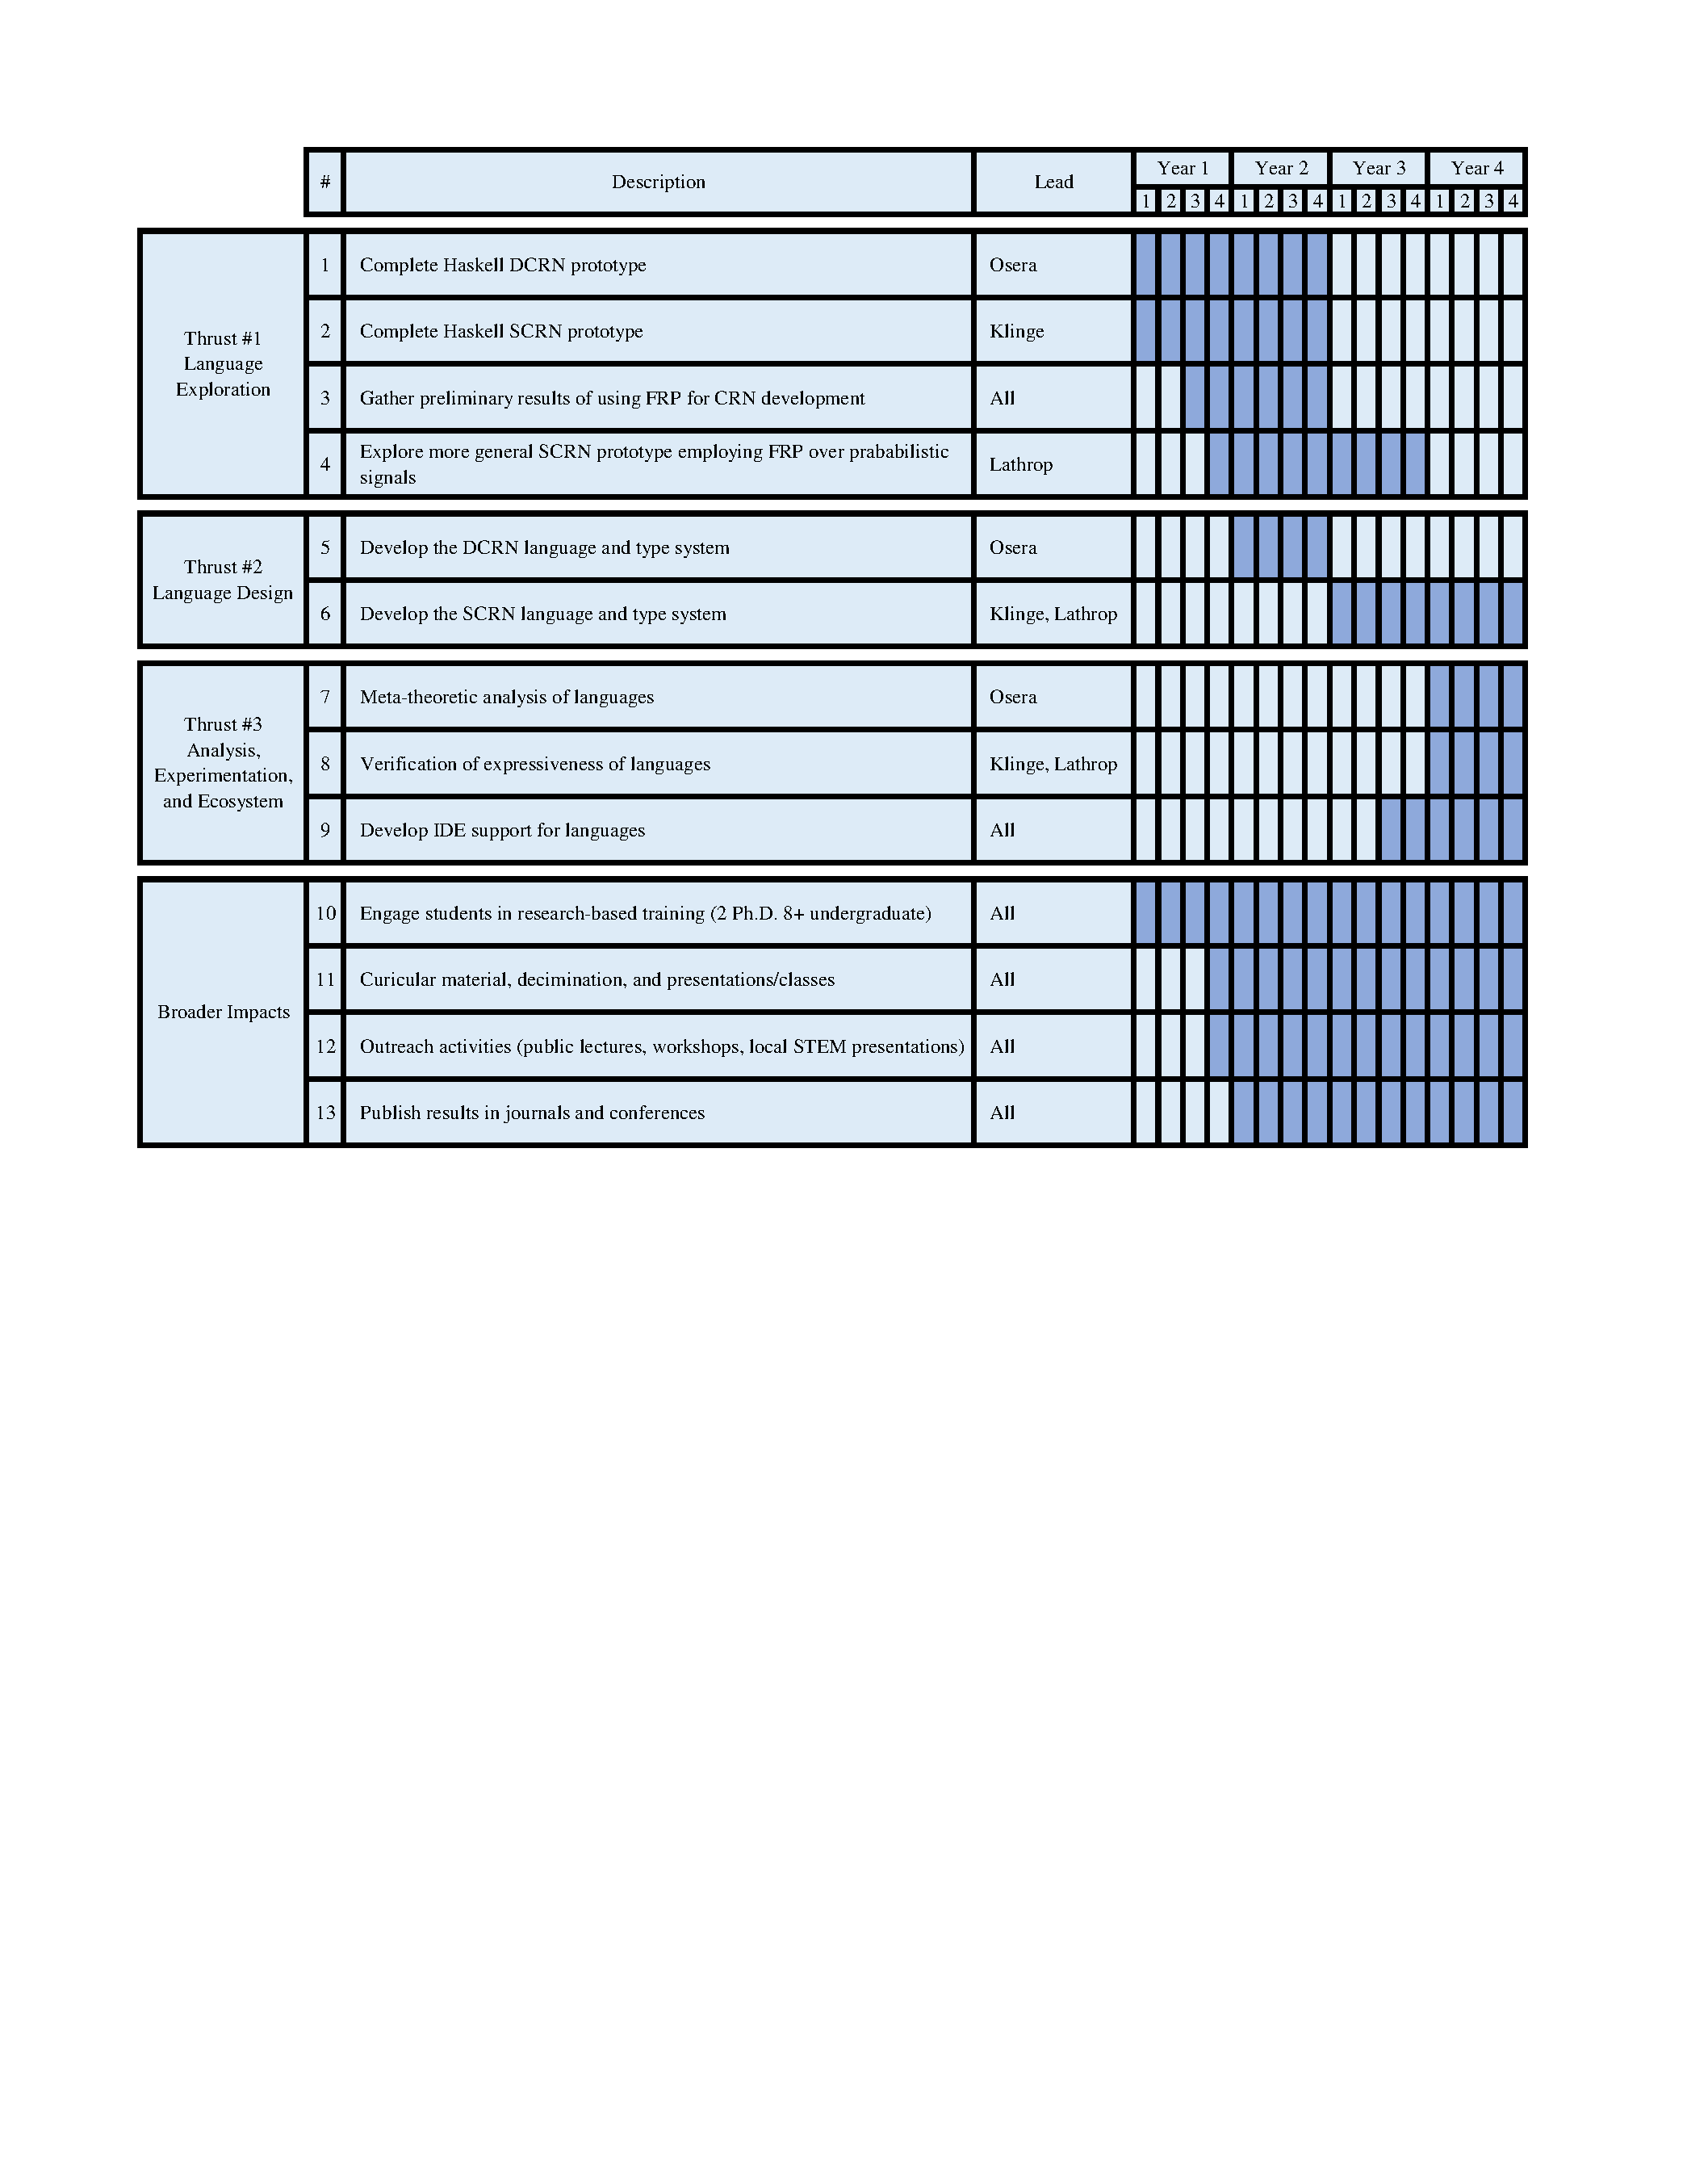
\includegraphics[width=6.4in]{TimeLine.pdf}
     \caption{Project Timeline}
 \end{figure}



    % %!TEX root = project_description.tex

\section{Results from Prior NSF Support}

{\bf J. Lathrop} is a Co-PI on the current award CNS 1545028, CPS:Synergy: Safety-Aware Cyber-Molecular Systems, 10/15/2015 -- 8/31/2020, \$823,930.

\subsection*{Intellectual Merit}
The project combines methods from computer science and software engineering with methods from molecular biology to gain insights into how to develop cyber-molecular systems that are safe for use in dynamic and only partially understood environments.
The project has developed a refined formulation of what robustness means in deterministic chemical reaction networks. to  perform correctly even when crucial physical parameters are perturbed by small amounts and shown that nondeterministic finite automata can be simulated by deterministic chemical reaction networks that are provably robust in this sense.  
The project found that the use of advanced requirements engineering techniques for cyber-molecular systems enabled earlier removal of obstacles to safe operations.  Key results from the project also include the development of chemical reaction network models for standard safety building blocks needed for cyber-molecular systems \cite{oKlLaLu15,  cElLaLu17, cElKlLa17, jEKLLLM17}.
The project also implemented and evaluated in the laboratory a DNA origami-based reconfigurable nanosystem with potential as a force/energy diagnostic tool \cite{jMatHen16, oMath16}.    Publications describing these and additional results include \cite{cKlin16,  cHuaStu16, jCaLuSt18, cElKlLa17,  jHKLLL18}.        

\subsection*{Broader Impacts}
Eight Ph.D. students have been supported or partially supported by this award. Five of these have graduated since 2016:  Samuel Ellis co-advised by J. Lathrop and R. Lutz (Ph.D. 2017, now a Software Scientist at the NSF-funded Molecular Sciences Software Institute), Titus Klinge advised by J Lathrop and J Lutz  (Ph.D. 2016, now an Assistant Professor at Drake University, and prior appointments as Visiting Assistant Professor at Grinnell College and Carleton College), Adam Case advised by J. Lutz (Ph.D. 2016, now an Assistant Professor at Drake University), Don Stull advised J. Lutz (Ph.D. 2017, now a Lecturer at Iowa State University, and prior appointment at INRIA), Divita Mathur advised by E. Henderson (Molecular Biology Department) and J. Lutz (Ph.D. 2016, now at the U.S> Navel Research Laboratory).  Four Ph.D. students currently work in the Laboratory for Molecular Programming (LAMP).  

The project's REU supported research by two outstanding students, Gabrielle Ortman (graduated 2017)  and Chase Koehler (graduated 2018; co-authored a paper \cite{cKMHL18}).

J. Lutz developed  an undergraduate/graduate course on molecular programming and has taught it seven times with help from J. Lathrop, who taught it an eighth time in Fall, 2018.  As part of our educational outreach, J. Lathrop, J. Lutz and R. Lutz mentor students on molecular programming projects at two local undergraduate institutions, Grinnell College and Simpson College.
The investigators gave three tutorials on cyber-molecular systems at conferences (ASE 2015, ICSE 2016, RE 2018); a workshop at Simpson College and two invited keynotes (RE 2016, SAFECOMP 2018).
R. Lutz also gave the invited, public Dean's 2017 Spring Lecture at Iowa State University. \\

\noindent{\bf P.M. Osera} was the PI on award CCF 1651817, EAGER: Semi-Automated Type-Directed Programming, 2016--2019, \$159,991.
%
\subsection*{Intellectual Merit}
This project investigated the foundations of type-directed program synthesis along two dimensions: (1) extending the foundations to handle advanced typing features such as polymorphism and generalized algebraic datatypes and (2) realizing the foundations in a semi-automated program synthesis tool, \textsc{Scythe}, that supports type-directed programming in the Haskell programming language.

\subsection*{Broader Impacts}
This project supported 12 undergraduates for summer research opportunities over its lifetime.
Three of the alumni from this project are either in or applying to doctoral programs in computer science and/or mathematics.
The project also funded their travel to present their work at Midwest PL Summit as well as attend the Programming Languages Mentoring Workshop at PLDI and ICFP.


    % %!TEX root = project_description.tex

\section{Temporary Place for CRN Examples}
\todo{Remove this section once it isn't needed (or move it elsewhere).}
This section is for generating motivating molecular programming examples that relate to this project.
(So this section will eventually need to be removed.)

\subsection{Hailstone Function}
Suppose we'd like to create a stochastic CRN that, given \( n \) initial molecules of type \( X \), will eventually produce \( H(n) \) molecules of type \( Y \) where \( H(n) \) is the Hailstone function:
\begin{equation}
    H(n) = \begin{cases}
        n/2, &\text{ if }n\text{ is even}\\
        3n+1, &\text{ if }n\text{ is odd}
    \end{cases}
\end{equation}
Computing this function with an SCRN can be broken into the following parts: (1) checking if \( n \) is divisible by two, (2) dividing \( n \) by two, (3) multiplying \( n \) by three, (4) incrementing a value by 1, and (5) multiplexing the output so that either \( n/2 \) or \( 3n+1 \) output depending on the result of the parity check.
Below is the SCRN that successfully computes this function:
\begin{align}
    X &\goesto{} A_\text{odd} + B + C + D\label{eq:hailstone_split}\\
    A_\text{odd} + A_\text{odd} &\goesto{} A_\text{even}\label{eq:hailstone_parity1}\\
    A_\text{even} + A_\text{even} &\goesto{} A_\text{even}\label{eq:hailstone_parity2}\\
    A_\text{odd} + A_\text{even} &\goesto{} A_\text{odd}\label{eq:hailstone_parity3}\\
    2 B &\goesto{} Y_1\label{eq:halstone_n2}\\
    C &\goesto{} 3Y_2\label{eq:halstone_3n}\\
    A_\text{even} + Y_1 &\goesto{} A_\text{even} + Y + \widehat{Y}_1\label{eq:halstone_mux1}\\
    A_\text{odd} + Y_2 &\goesto{} A_\text{odd} + Y + \widehat{Y}_2\label{eq:halstone_mux2}\\
    A_\text{odd} + Y + \widehat{Y}_1 &\goesto{} A_\text{odd} + Y_1\label{eq:halstone_rev1}\\
    A_\text{even} + Y + \widehat{Y}_2 &\goesto{} A_\text{even} + Y_2\label{eq:halstone_rev2}\\
    2 D &\goesto{} D\label{eq:halstone_1}\\
    D + \widehat{D} &\goesto{} D\\
    2Y + 2\widehat{D} &\goesto{} Y + \widehat{D}\\
    A_\text{odd} + D &\goesto{} A_\text{odd} + Y + \widehat{D}\\
    A_\text{even} + Y + \widehat{D} &\goesto{} A_\text{even} + D\label{eq:halstone_1end}
\end{align}
In the above SCRN, reaction~\eqref{eq:hailstone_split} simply copies the number of \( X \)'s into four species that can be used to compute all four components necessary to finish the algorithm in parallel.
Reactions~\eqref{eq:hailstone_parity1}--\eqref{eq:hailstone_parity3} compute the Boolean parity function: if \( n \) is even, then the number of \( A_\text{even} \)'s converges to 1 and the number of \( A_\text{odd} \)'s converges to 0; likewise, if \( n \) is odd, then \( A_\text{odd} \) goes to 1 and \( A_\text{even} \) goes to 0.
Reaction~\eqref{eq:halstone_n2} computes \( n/2 \) and stores the answer in \( Y_1 \).
Reaction~\eqref{eq:halstone_3n} computes \( 3n \) and stores the answer in \( Y_2 \).
Reactions~\eqref{eq:halstone_mux1}--\eqref{eq:halstone_mux2} uses the result of the parity check and copies \( Y_1 \) into \( Y \) if \( A_\text{even} \) exists and \( Y_2 \) is copied if \( A_\text{odd} \) exists.
These multiplexer reactions can be reversed using reactions~\eqref{eq:halstone_rev1}--\eqref{eq:halstone_rev2} so that any values copied over prematurely can be undone once the parity computation finishes.
Finally, reactions~\eqref{eq:halstone_1}--\eqref{eq:halstone_1end} are responsible for computing the number 1 and copying it into \( Y \) if \( n \) is odd.

\subsection{Maximum Function}
There has been some recent research on \emph{composable} SCRNs, \ie, SCRNs that can be modularly combined with provably no problems occurring~\cite{doty19}.
It is well-known that these SCRNs must be \emph{output-oblivious}, \ie, the number of output molecules must be generated in a monotonically increasing fashion.
It is also well-known that computing the \emph{maximum} of two numbers cannot be computed by an SCRN in an output-oblivious fashion.

For example, below is an implementation of maximum with an SCRN:
\begin{align}
    X_1 &\goesto{} A_1 + Y\\
    X_2 &\goesto{} A_2 + Y\\
    A_1 + A_2 &\goesto{} B\\
    Y + B &\goesto{} \emptyset
\end{align}
The idea behind the above solution is that we can write the maximum of two numbers \( n_1, n_2 \) as:
\[
    \text{max}(n_1, n_2) = n_1 + n_2 - \text{min}(n_1, n_2).
\]
We compute the maximum function in this way by first computing the sum of \( X_1 \) and \( X_2 \) and storing the result in \( Y \), and then later subtracting from \( Y \) the minimum of \( X_1 \) and \( X_2 \) (this is computed with the \( A_1 + A_2 \goesto{} B \) reaction.)

Notice that this is NOT computing \( Y \) in a monotonically increasing fashion.
We first compute the sum (which could overshoot the maximum by quite a lot), and later we will decrease the total number of \( Y \)'s using the \( Y + B \goesto{} \emptyset \) reaction.

\subsection{Signal Multiplexer}
CRNs don't need to be considered machines that take in natural numbers and output natural numbers.
In fact, they are more naturally a \emph{signal processor} and can receive streams of molecules, \ie, a time-varying signal of molecules, and output a time-varying signal of molecules in response.

As a simple case of this, consider a deterministic CRN implementation of a multiplexer that receives two signals as input through species \( X_1 \) and \( X_2 \) along with a switch molecule \( S \).
If \( S \) is close to 1, then we want to have the output \( Y \) be identical to the signal provided through \( X_1 \), and if \( S \) is close to 0, then we want to have \( Y \) be identical to the signal \( X_2 \).
This cannot be done with perfect accuracy, but here is an approach:
\begin{align}
    S + X_1 &\goesto{k} S + X_1 + Y\\
    \overline{S} + X_2 &\goesto{k} \overline{S} + X_2 + Y\\
    Y &\goesto{k} \emptyset.
\end{align}
This approximates what we want because the ODE for \( Y \) is:
\begin{equation}
    \frac{dy}{dt} = k\left[s(t)x_1(t) + \overline{s}(t)x_2(t) - y(t)\right].
\end{equation}
Now, if \( s(t) + \overline{s}(t) = 1 \) for all \( t\in[0,\infty) \), then when \( S \) is close to 1, then \( \overline{S} \) is close to 0 and vice versa.
Thus, the above equation is really equal to one of the following:
\begin{align}
    \frac{dy}{dt} = k\left[x_1(t) - y(t)\right]\\
    \frac{dy}{dt} = k\left[x_2(t) - y(t)\right]
\end{align}
Thus, if \( S \) is high, then \( Y \) is ``chasing'' the concentration of \( X_1 \), and if \( S \) is low, then \( Y \) is ``chasing'' \( X_2 \).
If \( k \) is sufficiently large, then \( Y \) is a great approximation of the multiplexer we desire.

The technique of splitting the signal \( S \) into two is called \textbf{dual-rail representation} which allows us to use the presence of \( \overline{S} \) to have the same meaning as the absence of \( S \).

\subsection{Use of an LTL-like Temporal Logic}
Many of the above examples have a \emph{specification} or \emph{requirement} that can easily be written in an LTL like language.
For example, the hailstone requirement would simply be the following:
\begin{equation}\label{eq:hailstone_ltl}
    \Diamond\Box\left[y = H(x(0))\right].
\end{equation}
Recall that \( \Diamond\Phi \) is the ``future'' operator and means that eventually \( \Phi \) becomes true and that \( \Box\Psi \) is the ``globally'' operator and means that \( \Psi \) must always be true.
Therefore, equation~\eqref{eq:hailstone_ltl} means: ``eventually the number of \( Y \)'s will be equal to \( H(x_0) \) forever,'' which is exactly what we want.

Similarly, the maximum function can be written in an LTL-like language like this:
\begin{equation}\label{eq:max_ltl}
    \Diamond\Box[y=\max(x_1(0),x_2(0))]
\end{equation}

One thing that should be noted, is that most interesting SCRNs only \emph{probabilistically} converge to the correct answer.
SCRNs can only compute the semi-linear functions with probability 1, but they are Turing universal if you allow for any \( \epsilon > 0 \) probability of failure.
Therefore, to quantify most SCRN requirements, such as computing \( 2^n \), the requirement would need to be specified probabilistically such as:
\begin{equation}
    \mathcal{P}_{\ge1-\epsilon}\Diamond\Box[y=2^{x(0)}]
\end{equation}
which says that with probability \( 1 - \epsilon \) the LTL formula must be true.

There are probabilistic logics that exist, such as \emph{probabalistic computational tree logic} (\emph{PCTL}) and \emph{continuous stochastic logic} (\emph{CSL}), however, these formulae are \emph{state} formulae instead of \emph{path} formulae like LTL.
Therefore, we expect using a probabilistic version LTL will be more useful.

For DCRNs, there is a temporal logical called \emph{signal temporal logic} which is a continuous-time, continuous-space, variant of LTL.
It specifies precise relationships between the input signals and output signals.
For example, we might write an STL formula for the DCRN signal processor specification mentioned above with:
\begin{equation}
    \Box[(s=1)\implies(y=x_1)]\land\Box[(s=0)\implies(y=x_2)],
\end{equation}
which means that globally, if \( s(t)=1 \) then the concentration of \( y(t) \) is equal to \( x_1(t) \), and similarly if \( s(t) = 1 \), then the concentration of \( y(t) \) is equal to \( x_2(t) \).
This is a VERY strict requirement because \( Y \) must \emph{exactly} equal the corresponding concentration of the input.
(It is easy to prove this is impossible for DCRNs.)
Thus, it would be better if we had a way of \emph{approximately} satisfying an STL formula.
For example, if we look at the solution to the system of ODEs that corresponds to the DCRN given, what we really want is to compute a \emph{distance measure} of how close we are to satisfying the STL formula and then say we \emph{\(\epsilon\)}-approximately satisfy it if the measure is within \emph{\(\epsilon\)}.

We have other previous results that use continuous stochastic logic (CSL) to specify requirements and then \emph{formally verify} their correctness in model checkers like PRISM.
In particular, these papers:~\cite{cEHKLLL14,tosem19}.
We specify the high-level requirements of a ``watchdog timer'' in CSL, refine them into smaller requirements, prove that the sub-goals imply the super-goals, and then use PRISM to verify the leaf goals of the requirements tree.


    % %\setcounter{page}{1}
    % \bibliographystyle{abbrv}
    % \bibliography{../preface/master}
    {\setbox0\vbox{\bibliography{../preface/master}}}

\end{document}
